\section{Problemas de práctica}

\subsection{Clasificación}



\begin{problema}
	Clasifica cada una de las siguientes ecuaciones diferenciales enunciando su orden; sus variables dependientes e independientes; y si es ordinaria o parcial:
	\begin{enumerate}
		\item
		\label{exmp 02_01}
		\begin{align*}
			\left(y''\right)^{2}+3x=2\left(y'\right)^3
		\end{align*}
		\item
		\label{exmp 02:02}
		\begin{align*}
			\dfrac{dy}{dx}+\dfrac{y}{x} = y^2
		\end{align*}
		\item
		\label{exmp 02:03}
		\begin{align*}
			\dfrac{d^{2}Q}{dt^{2}}-3\dfrac{dQ}{dt}+2Q = 4\sin(2t)
		\end{align*}
		\item
		\label{exmp 02:04}
		\begin{align*}
			\dfrac{dy}{dx}=\dfrac{x+y}{x-y}
		\end{align*}

		\item
		\begin{align*}
			(x+y)dx+(y-x)dy = 0
		\end{align*}
		\item
		\begin{align*}
			\dfrac{\partial^{2}V}{\partial x^{2}} +
			\dfrac{\partial^{2}V}{\partial y^{2}} = 0
		\end{align*}
	\end{enumerate}

\end{problema}

\subsection{Ecuaciones especiales}

\begin{problema}
	\begin{enumerate}[(i)]
		%NUEVO ITEM
		\item Encuentra la solución general de
		\begin{align*}
			\left( 4x+xy^{2} \right)dx+\left( y+x^{2}y \right)dy = 0
		\end{align*}

		\item Encuentra la solución particular para $y(1)=2$.
	\end{enumerate}
\end{problema}

\begin{problema}
	Resuelve el problema de valor inicial
\begin{align*}
	\begin{cases}
		\dfrac{dy}{dx}+3y=8 \\
		y(0)=2
	\end{cases}
\end{align*}
\end{problema}

\begin{problema}
	Resuelve la ecuación
	\begin{align*}
		\dfrac{dy}{dx} = \sec(y)\tan(x)
	\end{align*}
\end{problema}

\subsection{Aplicaciones}


\begin{problema}
	Un cuerpo a una temperatura de $50^{o}F$ está colocado en el exterior donde la temperatura es de $100^{o}F.$ Si después de 5 minutos la temperatura del cuerpo es $60^{o}F,$ encontrar:
	\begin{enumerate}
		\item cuanto le tomará al cuerpo alcanzar una temperatura de $75^{o}F$ y
		\item la temperatura del cuerpo después de 20 minutos.
	\end{enumerate}

\end{problema}

	\begin{problema}
	Un cuerpo que pesa \texttt{64lbs} es dejado caer desde una altura de \texttt{100fts} con velocidad inicial de \texttt{10ft/sec.}

	Suponga que la resistencia del aire es proporcional a la velocidad del cuerpo. Se sabe que la velocidad límite del cuerpo es de \texttt{128ft/sec}. Encuentre:
	\begin{enumerate}
		\item una expresión para la velocidad del cuerpo en cualquier tiempo $t$,  y
		\item una expresión para la posición del cuerpo en cualquier tiempo.
		\item Determine el instante en que choca contra el suelo.
	\end{enumerate}

\end{problema}


\begin{problema}
	Un tanque de 50 lts contiene inicialmente $10$ litros de agua fresca. Al tiempo $t=0$ se vierte al tanque una solución de salmuera que contiene $1$ kilo de sal por litro a un ritmo $4$ lts/min, mientras que la mezcla bien agitada abandona el tanque a un ritmo de $2$ lts/min. Encuentre
	\begin{enumerate}
		\item la cantidad de tiempo requerido para que ocurra un derrame y;
		\item la cantidad de sal en el tanque al momento del derrame.
	\end{enumerate}

\end{problema}

\begin{figure}
	\centering
	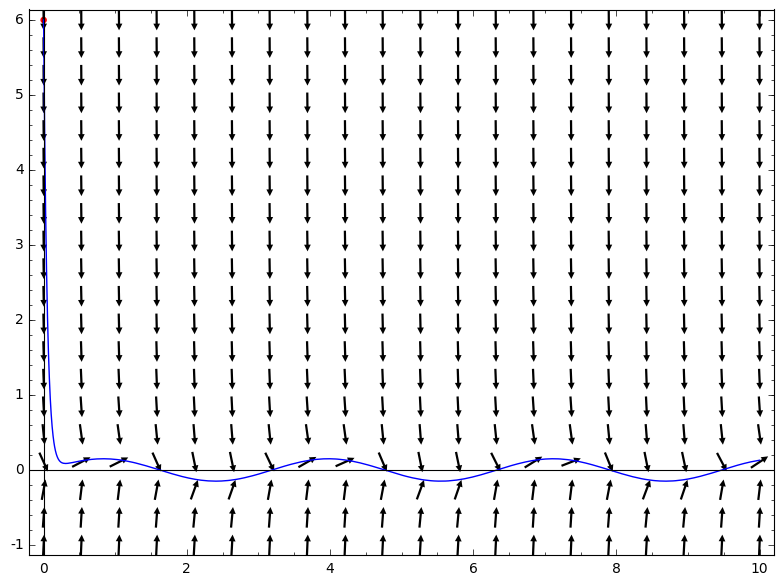
\includegraphics[height=5cm,keepaspectratio=true]{./edo/img020505.png}
	% img020504.png: 0x0 pixel, 300dpi, 0.00x0.00 cm, bb=
	\label{fig:020505}
\end{figure}

\begin{problema}
	Un circuito $RL$ tiene una $fem$ (en voltios) dada por $3sin(2t),$ una resistencia de 10 ohmios, una inductancia de 0.5 henrios y una corriente inicial de 6 amperios. Encuentre la corriente de estado estacionario.
\end{problema}



